


  



                          %%% SETS %%%
\chapter {Sets}

\section {Set Definition}
%This is only an introduction to set theory as originally presented by Georg Cantor, now known as naive set theory to set it apart from later work which attempts to put it onto an axiomatic basis. 

\begin {definition}
A \textit{set} is an unordered but well defined collection of objects which are called the \textit{elements/members} of the set.  The objects in a set are called the \textit{elements} or \textit{members}, of the set. A set is said to \textit{contain} its elements. We write $a \in A$ and say, ``a is an element of the set A'' to mean that $A$ contains $a$ and $a \notin A$ to mean that the element $a$ is not contained by the set $A$.
\end {definition}

\begin{notes}
   Sets are unordered. \{a, b\} is the same as \{b, a\}. The number of times an object is enumerated makes no difference, it is still one element.
\end{notes}


  \section{Set Specification}
    \subsection {Set Enumeration}
  The easiest way to describe small sets is to enumerate (list) the elements. This is done by writing the elements between braces with a comma between them. For example let $V$ be the set of English vowels. We can write $V=\{a,e,i,o,u\}$ to define the set $V$. If we want to talk about the positive odd integers less than 10 as the set $O$, we can define it as the set $\{1,3,5,7,9\}$. 
The set $M=\{1, "1", \text{my dog Rover}, \text{red-head}\}$ can be a set. The notation $a_1,a_2,a_3 \in A$ is the same as $a_1 \in A, a_2 \in A, a_3 \in A$. We can start a pattern and use the ellipses symbol to indicate that the reader should infer the pattern. R=\{3,6,9,12,15, \dots\}. $\{0,1,2,3, \dots ,100\}$ The enumeration can be a description of the elements. \{addresses on Pine Street\} defines a set of addresses that are on Pine Street. $O=\{ \text{positive odd integers less than 10} \}$. 


     \subsection {Set Builder Notation}
Set comprehension, set intension. Three parts, a variable, a colon or vertical bar and a logical predicate.  


$\{a | \text{  a is a positive integer }\} $

or 

$E: \text{is even}$, 
$A= \{a | E(a)\}$\\
We read this as 
set A is defined as the set of all $a$ such that $a$ is even. The vertical bar is read "such that". To the left are the variables that represent the set members and to the right is the condition that all members must satisfy.

Example: $A = \{x | \lnot E(x),x<10\}  $

\begin{notes}
Predicates separated by commas are implied conjunction.
\end{notes}
  
Sometimes we restrict the domain of a quantified statement explicitly by making use of a particular notation. For example, $\forall x \in S (P(x))$       %∀x∈S(P(x)) 
denotes the universal quantification of $P(x)$ over all elements in the set $S$. In other words, $\forall x \in S (P(x))$  is shorthand for $\forall x (x \in S(P(x)) \rightarrow P(x))$    
%∀x∈S(P(x)) is shorthand for ∀x(x ∈ S → P(x)).
Similarly, $\exists x \in S(P(x))$ denotes the existential quantification of $P(x)$ over all elements in $S$. That is, $\exists x \in S(P(x))$ is shorthand for $\exists x (x \in S \land P(x))$.
%Similarly, ∃x∈S(P(x)) denotes the existential quantification of P(x) over all elements in S.
%That is, ∃x∈S(P(x)) is shorthand for ∃x(x ∈ S ∧ P(x)).


\section {Common sets and their Notation in Mathematics and Computer Science}
 $\mathbb{N}=\{1,2,3, \dots \} \text {the set of \textbf{natural numbers} } $ \\
 $\mathbb{Z}=\{\dots -3,-2,-1,0,1,2,3, \dots\}  \text{The set of } \textbf{integers}$ \\
 $\mathbb{Q}=\{\dfrac{p}{q} | p \in \mathbb{Z}, q \in \mathbb{Z}, q \neq 0 \} \text{The set of \textbf{rational numbers}}$ \\
 $\mathbb{R}=\{ \text{the set of }\textbf{real numbers}   \} $ \\
 $\mathbb{C}=\{ \text{the set of }\textbf{complex numbers} \} $ \\
 $\mathbb{B}=\{0,1\} \text{ the set of \textbf{a set of binary symbols} } $ \\
 





\begin {notes}
 We can restrict the universe from which the objects are drawn to the right of the "$|$" like so: \\
 $O=\{\mathbb{Z}^+ | x \text{ is odd and } x<10 \}$  \\
This is read as "The set O is equal to the set of all x drawn from the set of positive integers such that x is less than 10."
The superscript indicates that only the positive members of the domain are to be considered.
Zero may or may not be considered a natural number depending upon the author. For this course we accept zero as a natural number and use the notation $\mathbb{Z}^+$ for the set of positive integers. The special font used for these special sets is called Blackboard Bold. Z is used for integers because the German word for numbers is Zahlen.
\end{notes}

  A set is an object. Therefore we can have a set which contains other sets:
  $$ \text{Basic data types} = \{\mathbb{B}, \mathbb{N}, \mathbb{Z}, \mathbb{R} \}$$
This fact leads to interesting paradoxes which mark the difference between what is known as Naive Set Theory and more advanced forms.

\begin{notes}
Sets and data types in programming languages are related.\\
There is a shortcut used sometimes to assert a universal truth for a set. For example $\forall x \in S(P(x))$ which asserts that all elements of the set $S$ have property $P$. It can also be stated as $\forall x(x \in S \rightarrow P(X))$
\end{notes}

\section {Truth Sets}
\begin {definition}[Truth Sets]\index{truth set}
Given a predicate $P$, and a domain $D$, we define the \textbf{truth set} of $P$ to be the set of elements $x$ in $D$ for which $P(x)$ is true. The truth set of $P(x)$ is denoted by$ \{ x \in D | P(x) \} $.
\end {definition}

  
\section {Set Equality}
\begin {definition}[Set Equality]\index{set equality}
Two sets are \textit{equal} if and only if they have the same elements. That is, if $A$ and $B$ are sets, then $A$ and $B$ are equal if and only if $\forall x(x \in A \leftrightarrow x \in B)$. We write $A=B$ if $A$ and $B$ are equal sets.
\end {definition}
\begin{notes}
Some authors will use $\subset$ specifically to designate a proper subset and use $\subseteq$ for subsets that could be equal. We only use $\subset$ in these notes to indicate either a proper subset or an equal set.
\end{notes}
  
\begin{definition}[Empty Set]\index{empty set}
A set that contains no elements is called \textit{null set} or \textit{empty set}and is denoted by $\emptyset$. The empty set can also be denoted by $\{ \}$
\end{definition}

\section{Subsets}
  If a set is composed of elements of another set, we call the new set a \textbf{subset}. The subset may have all the same elements as the first set. If it has fewer elements, we may call it a \textbf{proper sub-set}.
  
\begin {definition}[Subset]\index{subset}
A set $A$ is said to be a \textit{subset} of $B$ if and only if every element of $A$ is also an element of $B$.  We write $A \subset B$ to indicate that $A$ is a subset of $B$ and $A \not\subset B$ to indicate that $A$ is not a subset of $B$. $\forall x(x \in A \rightarrow x \in B)$ is true whenever $A$ is a subset of $B$.
\end {definition} 

\begin {theorem}
$A=B$  if and only if $A \subset B$ and $B \subset A$
\end {theorem}

 \subsection{Intervals of Reals}  
  We frequently talk about subsets of the reals or integers  as intervals. There are conflicting notations.

\begin{align*}
 \big( a,b\big) = &\big] a,b\big[ &= \{ x \in \mathbb{R}   |   a < x < b       \}, \\
 \big[a ,b\big) = &\big[ a,b\big[ &=  \{ x \in \mathbb{R}  | a \le x<b      \}, \\
 \big(a ,b\big] = &\big] a,b\big] &=  \{ x \in \mathbb{R}  | a < x \le b       \}, \\
 \big[ a,b\big] = &\big[ a,b\big]  &=  \{ x \in \mathbb{R} | a \le x \le  b  \}.
\end{align*}
For intervals that extend to infinity toward the negative or positive infinity, we substitute $-\infty$ for $a$ or $+\infty$ for $b$.

 \subsection{Integer Intervals}
 The notation $\big[ a \ldots b\big] $ when $a$ and $b$ are integers, or $\big\{a\ldots b\big\}$ , or just $a\ldots b$ is sometimes used to indicate the interval of all integers between $a$ and $b$, including both. This notation is used in some programming languages; in Pascal, for example, it is used to formally define a subrange type, most frequently used to specify lower and upper bounds of valid indices of an array.
 
 An integer interval that has a finite lower or upper endpoint always includes that endpoint. Therefore, the exclusion of endpoints can be explicitly denoted by writing $a\ldots b-1$,$a+1\ldots b$, or $a+1\dots b-1$. Alternate-bracket notations like $[a\ldots b)$ or $[a\ldots b[$ are rarely used for integer intervals.

\begin{definition}
We denote the set $\{0,1,\dots m-1\}$ with the notation $\mathbb{Z}_m$.
\end{definition}

  
\section {Universal and Empty Sets}
\begin {definition}[Universal and Empty Sets]\index{universal set} \index{empty set}
The \textit{universal set} or universe is a set that represents some domain of discourse. There is no symbol that everyone accepts as the symbol for the universal set. We adopt $\mathbb{U}$ to designate the universal set.
The set which contains no elements is the \textit{null} or \textit{empty set} and is disignated by $\emptyset$. 
\end {definition}

\begin{notes}
Never confuse $\emptyset$ with \{$\emptyset$\}. The first is a set which contains no elements. The second is a set which contains one element and that element is a set which contains no elements. Think of file folders on a disk as sets and files as elements.
\end{notes}

 \begin {theorem}
For any set S, the following are true:\\
$\emptyset \subset S$ , \\
$S \subset \mathbb{U}$, \\
$\emptyset \text{ is unique}$\\
For any set $S, \emptyset \subset S \subset \mathbb{U}$
\end {theorem}


\section {Set Operators}

\begin {definition} [Set Union]\index{set union}
Let $A$ and $B$ be sets. The \textbf{union} of the sets $A$ and $B$, denoted by $A \cup B$, is the set that contains those elements that are either in $A$ or in $B$, or in both. $A \cup B=\{x:x \in A \lor x \in B\}$
\end {definition}

\begin{figure}[htbp]
   \centering
   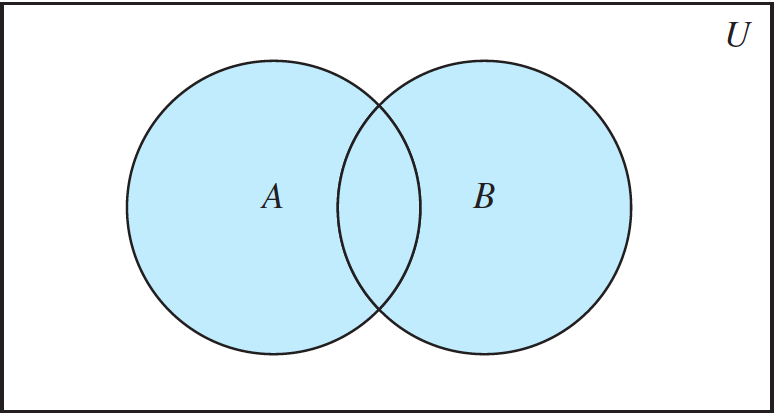
\includegraphics [width=3in]{Figure-2-2-1-VennDiagramOfAUnionB}
   \caption{Venn Diagram Of A Union B}
   \label{figure:Venn Diagram Of A Union B}
\end{figure}
   
\begin {definition}[Set Intersection]\index{set intersection}
Let $A$ and $B$ be sets. The \textbf{intersection} of the sets $A$ and $B$, denoted by $A \cap B$, is the set containing those elements in both $A$ and $B$.
$A \cap B = \{x:x \in A  \land x \in B\}$
\end {definition}

\begin{figure}[htbp]
   \centering
   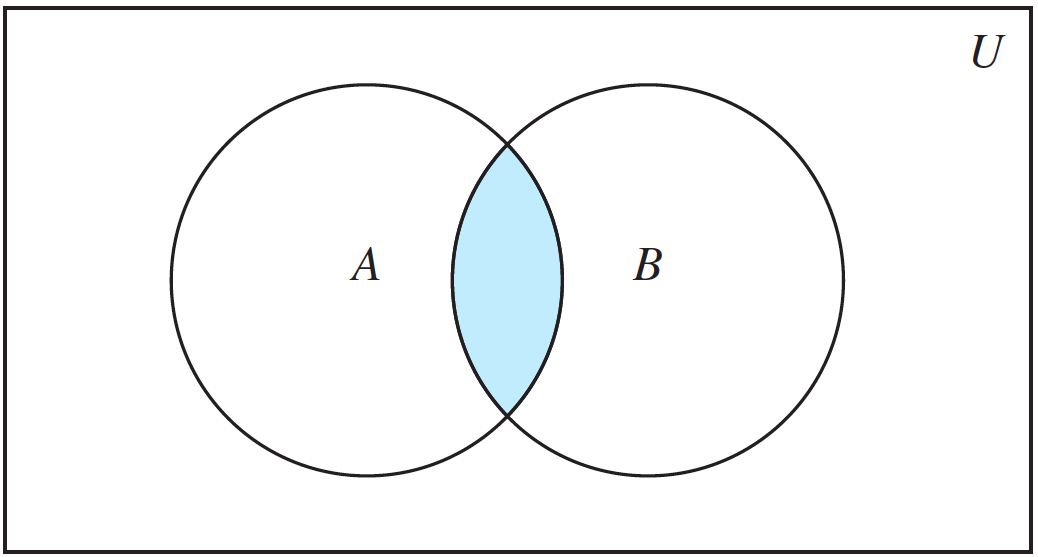
\includegraphics [width=3in]{Figure-2-2-2-VennDiagramOfTheIntersectionOfAandB}
   \caption{Venn Diagram Of The Intersection Of A and B}
   \label{figure:Venn Diagram Of The Intersection Of A and B}
\end{figure}

\begin {definition}[Disjoint Sets]\index{disjoint sets}
Two sets are disjoint if and only if $A \cup B = \emptyset$
\end {definition}

\begin {definition}[Set Difference]\index{set difference}
Let $A$ and $B$ be sets. The \textit{difference} of $A$ and $B$ denoted by $A - B$ and sometimes by $A \setminus B$ according to the ISO 31-11 standard, is the set containing those elements that are in $A$ but not in $B$. The difference of $A$ and $B$ is also called the \textit{complement of B with respect to A}.
$A - B = \{x | x \in A \land x \notin B\}$.
\end {definition}

 It is sometimes written $B - A$, but this notation is ambiguous, as in some contexts it can be interpreted as the set of all elements $b - a$, where b is taken from B and a from A.

\begin{definition}[Symmetric Difference]\index{symmetric difference}
The symmetric difference of $A$ and $B$, denoted by $A \oplus B$, is
the set containing those elements in either $A$ or $B$, but not in
both $A$ and $B$.
\end{definition}

\begin {definition} [Set Complement]\index{Set Complement}
$A^C$ or $ \bar{A} $ is called a set complement. It is all elements of the universal set which are not contained in the set $A$.
\end {definition}

\section {Identities of Set Algebra}
Set operators give identities that can be proven. The following are a list of the most basic identifies and the names they are given. Any of these can be proven using the formal definition of the operator and the rules of equivalence and inference from logic.


   \begin{table}[htbp]
   \centering
   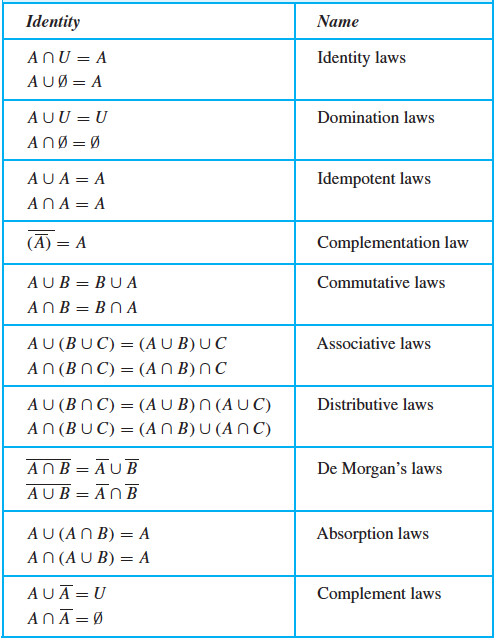
\includegraphics [scale=0.5]{Table-2-2-1-SetIdentities}
   \caption{Set Identities}
   \label{table:Set Identities}
   \end{table}


\begin{notes}
Note the similarity to Identities of Logic 
\end{notes}

\section {Venn Diagrams}
    Diagrams that represent sets as ovals within a square box with or without labeled elements are called Venn diagrams. The outer box represents the universe of discourse, $U$, for the sets.   In a Venn diagram, the universal set is th einterior of a rectangle. If $A \subset B$, then the area of $A$ will be contained within the area of $B$.
If $A$ and $B$ are disjoint, then the area of $A$ will overlap art of the area of $B$.

   \begin{table}[htbp]
   \centering
   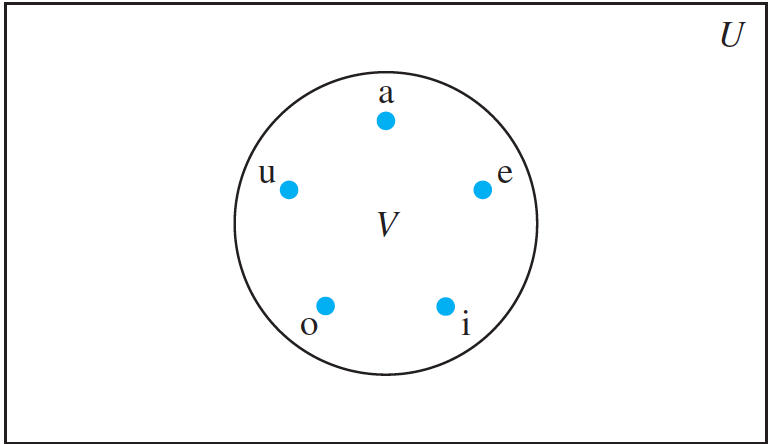
\includegraphics [width=2in]{Figure-2-1-1-VennDiagramOfVowels}
   \caption{VennDiagramOfVowels}
   \label{figure:VennDiagramOfVowels}
   \end{table}



    \begin{definition}[Set Cross Product or Cartesian Cross Product]\index{set cross product}
The ordered n-tuple $(a_1, a_2, . . . , a_n)$ is the ordered collection that has $a_1$ as its first element, $a_2$ as its second element, . . . , and $a_n$ as its $n$th element.
Two tuples are considered equal if and only if all corresponding elements of the two tuples match.

$$A \times B = \{(a,b)\mid a \in A \land b \in B\}$$
    \end{definition}

    \begin{definition}
    Let $A$ and $B$ be sets. The Cartesian product of $A$ and $B$, denoted by $A \times B$, is the set of all
ordered pairs $(a, b)$, where $a \in A$ and $b \in B$. Hence,
$A \times B = \{(a, b) \vert a \in  A \land b \in B\}$.
    \end{definition}
    
$A \times B$
\begin{notes}
The elements of a tuple are ordered. $(a,b)$ is not the same as $(b, a)$.\\
Cross products of sets to themselves can be represented with superscripts. $A^2=A \times A$.\\
The cross product is a SET of TUPLES.
\end{notes}

    \begin {definition}
    The Cartesian product of the sets $A_1,A_2, . . . , A_n$, denoted by $A_1 \times A_2 \times \dots \times A_n$, is the
set of ordered n-tuples $(a_1, a_2, . . . , a_n)$, where $a_i$ belongs to $A_i$ for $i$ = 1, 2, . . . , n. In other
words,
$A_1 \times A_2 \times \dots \times A_n = \{(a_1, a_2, . . . , a_n) | a_i \in A_i$ for $i = 1, 2, . . . , n\}$.
    \end {definition}

\section {Set Cardinality}
\begin {definition}[Set Cardinality]\index{set cardinality}
The size of the set is the number of elements in the set for sets with a finite number of elements. We will defer infinite sets until later. This is called the set \textit{cardinality}. It is denoted by $\mathbf{card}(S)$ or $|S|$.
\end{definition}

\begin{definition}[Powerset]\index {powerset}
A special set called the power set is that set which includes every possible and unique subset of some set $S$. 
Note: the easiest way to enumerate the subset is by the number of elements in the set. List all the subsets with zero members (only one, the null set). Then all the subsets of size 1, 2, etc. 
\end{definition}
\begin {theorem}
If the size of set $S$ is $m$, there are $2^m$ posible subsets.
\end{theorem}

Special symbol  $\mathcal{P} (A)$ designates the power set of set A.

\begin{notes}
the powerset IS A SET of SETS
\end{notes}


\section {Indexed Sets/Indexed Classes of Sets and Generalized Set Operations }
%NOTE: the requires functions!!
Let $I$ be any nonempty set (not necessarily a numeric set), and let $S$ be a collection of sets. An indexing function from $I$ to $S$ is a function $f:I \rightarrow S$. For an $i \in I$, we denote the image $f(i)$ by $A_i$. Thus we can say:

$\{A_i : i \in I\} or \{A_i\} \in I$, or simply $\{A_i\}$

The set $I$ is called the \textbf{indexing set} and the elements of $I$ the \textbf{indices}. 

When many sets are joined or intersected, we introduce an indexed notation:


$\cup _{ i=1} ^ n a _{i}$

$\cap_{ i=1} ^ n a _{i}$


(give Venn diagram)

Representations of sets, set membership tables.


\begin{definition}[Fundamental Product of Sets]\index {Fundamental Products of Sets}
Consider a set of sets $A_1$, $A_2$, etc that are all unique. 
Now let $A_i^*$ mean either $A_i$ or  $A_i^c$, that the notation $A_i^*$ either means $A_i$ or it means $A_i^c$.
The fundamental product of the set $S$ is that is the union of all sets denoted by $A^*$
\end{definition}
\begin{notes}
there are m sets, $2^n$ such fundamental products (why?)
any two fundamental products are disjoint
the union of all the fundamental products is the universal
\end{notes}



\begin{definition}[Partitions of a Set]\index{partitions of a set}
A \textbf{partition} of a set $S$ is a collection of disjoint nonempty subsets of $S$ that have $S$ as their union. Equivalently we can say the collection of subsets $A_i$, $i \in I$ where $I$ is an index set) forms a partition if and only if
$$A_i \neq \emptyset \text{  for  } i \in I$$
$$A_i \cup A_j =  \emptyset \text{  when  } i \neq j$$
$$\bigcup_{i \in I} A_i = S$$
\end{definition}

\section {Multisets and Bags}\index{multiset} \index{bag}
A \textit{multiset} is a set that does not require each object to be unique. It can be represented by a set of pairs with the first element of the pair representing the object and the second representing the \textit{multiplicity} of that object in the multiset. These are sometimes called \textit{bags}

Sometimes the number of times that an element occurs in an unordered collection matters. Multisets are unordered collections of elements where an element can occur as a member more than once. The notation $\{m_1 \cdot a_1, m_2 \cdot a_2, \dots ,m_r \cdot a_r\}$ denotes the multiset with element $a_1$ occurring $m_1$ times, element $a_2$ occurring $m_2$ times, and so on. The numbers $m_i, i=1,2,3, \dots r$ are called the multiplicies of the elements $a_i, i=1,2,3, \dots ,r$.

%Sometimes the number of times that an element occurs in an unordered collection matters. Multisets are unordered collections of elements where an element can occur as a member more than once. The notation {m1 · a1, m2 · a2, . . . , mr · ar } denotes the multiset with element a1 occurring m1 times, element a2 occurring m2 times, and so on. The numbers mi , i = 1, 2, . . . , r are called the multiplicities of the elements ai , i = 1, 2, . . . , r.

\section{Strings}\index{string}
We noted that a set cross product may not have a numeric sets but may map to some arbitrary set of symbols. The set of English letters can be the set. If we let the symbol $\Sigma$ represent a set of unique symbols then we can represent the set of all pairs as $\Sigma^2$, all triples as $\Sigma^3$, etc and we call $\Sigma$ an \textbf{alphabet}. We can extend this concept to a set of strings that do not all need to be the same length. Since members of $\Sigma$ are distinct and unique, there is no ambiguity in dropping the parentheses when representing the set of strings. 

Strings have some special notation and definitions. The string that contains no elements is the empty string, represented by a lower case lambda, $\lambda$. A string may be called a word.





    \subsection {Kleene Star notation}\index{Kleene Star}
Sometimes we wish to discuss all the possible strings that could be constructed  We can construct exactly one sequence of length zero from a alphabet $\Sigma$ which we represent as $\lambda$. If the domain of the sequence has $m$ elements, it is possible to construct $m$ strings (words) of length 1, $m^2$ of length 2, $m^3$ of length 3, etc. We will often want to talk about strings that can be of any length but only contain elements drawn from the codomain. This will be the union of the set of length zero, the sets of length 1,2,3, ... to infinity. This set of all possible strings drawn from the set is called the Kleene closure and designated $K_*$

We can talk about binary numbers as strings. 
$\mathbb{B}^2$ designates the set of binary strings of two bits.  \{00,01,10,11\}\\
$\mathbb{B}^8$ designates the set of 8 binary strings $\{00000000, 00000001, 00000010, \dots ,11111111\}$ \\
$\mathbb{B}^*$ represents the set of all possible binary strings.

\section{From Paradox to Types}
A point that is much better addressed in an advanced class is the fact that the naive theory of sets is bounded by Russell's paradox. To avoid that paradox in programming languages there is a theory of types which permeates programming languages. We make the notational observation here which is used for the remainder of the text. Each variable is drawn from some set. The convention which is largely adopted is to place that set, which we call type, following the declaration of the variable like so: \textit{operand1:real} to designate that the variable \textit{operand1} is understood to contain a number drawn from $\mathbb{R}$. However we quickly get beyond mathematical sets in this text to define variables like $S:graph$ where $graph$ is understood to be a set/type of mathematical graph. 

\newpage
